\documentclass[
11pt, % The default document font size, options: 10pt, 11pt, 12pt
%codirector, % Uncomment to add a codirector to the title page
]{charter} 


% El títulos de la memoria, se usa en la carátula y se puede usar el cualquier lugar del documento con el comando \ttitle
\titulo{Desarrollo de un sistema basado en herramientas de visión por computadoras para la recomendación de recetas a partir de fotos de alimentos} 

% Nombre del posgrado, se usa en la carátula y se puede usar el cualquier lugar del documento con el comando \degreename
%\posgrado{Carrera de Especialización en Sistemas Embebidos} 
%\posgrado{Carrera de Especialización en Internet de las Cosas} 
\posgrado{Carrera de Especialización en Inteligencia Artificial}
%\posgrado{Maestría en Sistemas Embebidos} 
%\posgrado{Maestría en Internet de las cosas}

% Tu nombre, se puede usar el cualquier lugar del documento con el comando \authorname
% IMPORTANTE: no omitir titulaciones ni tildación en los nombres, también se recomienda escribir los nombres completos (tal cual los tienen en su documento)
\autor{Ing. Fabricio Denardi}

% El nombre del director y co-director, se puede usar el cualquier lugar del documento con el comando \supname y \cosupname y \pertesupname y \pertecosupname
\director{Dr. Ing. Facundo Adrián Lucianna}
\pertenenciaDirector{FIUBA} 
\codirector{} % para que aparezca en la portada se debe descomentar la opción codirector en los parámetros de documentclass
\pertenenciaCoDirector{FIUBA}

% Nombre del cliente, quien va a aprobar los resultados del proyecto, se puede usar con el comando \clientename y \empclientename
\cliente{Ing. Sebastián Camjayi}
\empresaCliente{FIUBA}
 
\fechaINICIO{15 de octubre de 2024}		%Fecha de inicio de la cursada de GdP \fechaInicioName
\fechaFINALPlan{3 de diciembre de 2024} 	%Fecha de final de cursada de GdP
\fechaFINALTrabajo{30 de junio de 2025}	%Fecha de defensa pública del trabajo final


\begin{document}

\maketitle
\thispagestyle{empty}
\pagebreak


\thispagestyle{empty}
{\setlength{\parskip}{0pt}
\tableofcontents{}
}
\pagebreak


\section*{Registros de cambios}
\label{sec:registro}


\begin{table}[ht]
\label{tab:registro}
\centering
\begin{tabularx}{\linewidth}{@{}|c|X|c|@{}}
\hline
\rowcolor[HTML]{C0C0C0} 
Revisión & \multicolumn{1}{c|}{\cellcolor[HTML]{C0C0C0}Detalles de los cambios realizados} & Fecha      \\ \hline
0      & Creación del documento                                 &\fechaInicioName \\ \hline
1      & Se completa hasta el punto 5 inclusive                & {28} de {octubre} de 2024 \\ \hline
2      & Se completa hasta el punto 9 inclusive				   & {4} de {noviembre} de 2024\\ \hline
%		  Se puede agregar algo más \newline
%		  En distintas líneas \newline
%		  Así                                                    & {día} de {mes} de 202X \\ \hline
3      & Se completa hasta el punto 12 inclusive                & {11} de {noviembre} de 2024 \\ \hline
4      & Se completa hasta el punto 15 inclusive                                & {18} de {noviembre} de 2024 \\ \hline

% Si hay más correcciones pasada la versión 4 también se deben especificar acá

\end{tabularx}
\end{table}

\pagebreak

\section*{Acta de constitución del proyecto}
\label{sec:acta}

\begin{flushright}
Buenos Aires, \fechaInicioName
\end{flushright}

\vspace{2cm}

Por medio de la presente se acuerda con el \authorname\hspace{1px} que su Trabajo Final de la \degreename\hspace{1px} se titulará ``\ttitle'' y consistirá en la implementación de una aplicación para dispositivos celulares que detecte los alimentos en una foto y recomiende recetas a partir de estos. El trabajo tendrá un presupuesto preliminar estimado de 601 horas y un costo estimado de ARS 65.312.170, con fecha de inicio el \fechaInicioName\hspace{1px} y fecha de presentación pública el \fechaFinalName.

Se adjunta a esta acta la planificación inicial.

\vfill

% Esta parte se construye sola con la información que hayan cargado en el preámbulo del documento y no debe modificarla
\begin{table}[ht]
\centering
\begin{tabular}{ccc}
\begin{tabular}[c]{@{}c@{}}Dr. Ing. Ariel Lutenberg \\ Director posgrado FIUBA\end{tabular} & \hspace{2cm} & \begin{tabular}[c]{@{}c@{}}\clientename \\ \empclientename \end{tabular} \vspace{2.5cm} \\ 
\multicolumn{3}{c}{\begin{tabular}[c]{@{}c@{}} \supname \\ Director del Trabajo Final\end{tabular}} \vspace{2.5cm} \\
\end{tabular}
\end{table}




\section{1. Descripción técnica-conceptual del proyecto a realizar}
\label{sec:descripcion}
En ocasiones, muchas personas  no saben qué cocinar y terminamos acudiendo a un delivery o a alimentos preprocesados que no son de nuestro agrado o no se adecuan a nuestra dieta.

La aplicación a desarrollar proveerá distintas alternativas de recetas para que el usuario pueda realizar su propia comida de acuerdo a sus especificaciones y deseos, con los alimentos que en ese momento posee.


Algunas heladeras \textit{smart} de alta gama ya disponen de esta funcionalidad. El principal problema es que estas heladeras suelen ser costosas. El valor agregado de esta aplicación es que solo se necesitará de un dispositivo móvil para tal fin.  \\ \\
A continuación se muestra un ejemplo de una foto que se utilizaría para detectar los alimentos y así recomendar recetas que los utilicen:
\label{sec:HeladeraEjemplo}


\begin{figure}[H]
\centering 
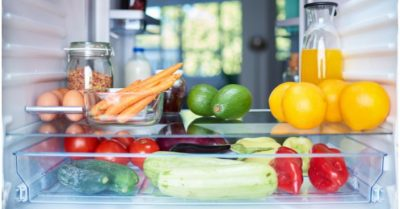
\includegraphics[width=.4\textwidth]{./heladera.jpg}
\caption{Ejemplo de \textit{input} para la detección de alimentos.}
\label{fig:HeladeraEjemplo}
\end{figure}


Se espera que la aplicación cuente con los siguientes módulos: 

\textbf{\textit{App Mobile} para la interacción con el usuario}\\
Con una interfaz sencilla, la aplicación deberá proveer las siguientes funcionalidades:
\begin{enumerate}
\item Captura de fotos de alimentos/heladeras con la que se obtendrá la recomendación.
\item Envío y recepción de las recomendaciones.
\item Visualización de las recetas que la aplicación sugiere al usuario.
\end{enumerate}

Si bien la idea es hacerlo multiplataforma, se espera, en principio, implementarlo para Android o IOS (una de las 2). Asimismo, se propone la utilización de \textit{frameworks} de desarrollo multiplataforma (como por ejemplo Flutter) para poder extenderlo a futuro.
  
\textbf{Detección de alimentos}\\
La recomendación cuenta con 2 partes:
\begin{enumerate}
\item Detección de alimentos en las fotos enviadas por los usuarios.
\item  La API proveerá una serie de métodos para devolver las recomendaciones solicitadas por el usuario.
\end{enumerate}

En principio, se utilizarían \textit{Transfer Learning} sobre modelos sobradamente probados y utilizados, como YOLO v8. Se deberá contemplar en la gestión de costos, el licenciamiento en caso de ser necesario.

\textbf{Recomendación de recetas}\\
En esta primera etapa se espera que la recomendación de las recetas se lleve a cabo a través de la API de Chat GPT. Aquí también se tendrá que tener en cuenta el costo de la licencia por el uso de la API de Chat GPT. \\

\textbf{Entrenamiento del modelo}\\
El entrenamiento del modelo de visión por computadora se realizará en un módulo aparte. Dicho módulo proveerá un paquete entrenado que la API utilizará.

\textbf{Módulos opcionales}\\
Se establecen los siguientes módulos que se incluirán o no de acuerdo a la gestión de alcance que se efectuará durante el cursado de la asignatura de gestión de proyectos.
\begin{enumerate}
\item Gestión de preferencias\\
El sistema recordará y valorará las preferencias del usuario para recomendar recetas. Para eso, habrá que implementar valoraciones de recetas personalizadas.

\item Retroalimentación \\
La app mobile dispondrá de una funcionalidad para permitir la retroalimentación, recuperando falsos positivos y negativos y así reentrenar el modelo con nueva información al respecto. 
\end{enumerate}

\textit{Disponibilidad de datos}\\
Si bien no se cuenta aún con un \textit{dataset} para entrenar el modelo de visión por computadoras que dará lugar a esta aplicación, en un análisis preliminar, hay disponibles diferentes conjuntos de imágenes con heladeras, alimentos, platos, que harán factible este proyecto. \\

A continuación se presenta un diagrama básico de los módulos que incluirá la aplicación. Notesé que los módulos no incluidos inicialmente se marcan en línea punteada:
\label{sec:DiagramaGeneral}

\begin{figure}[H]
\centering 
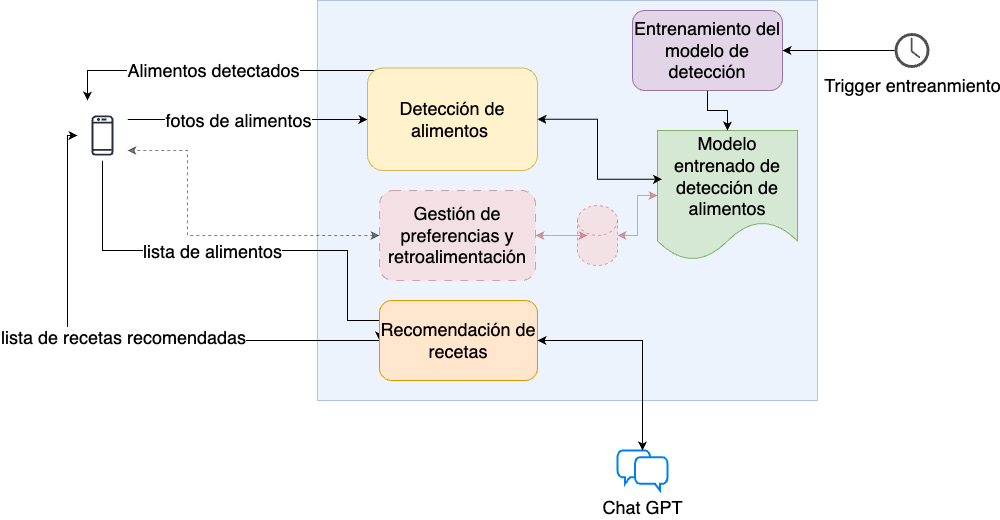
\includegraphics[width=.8\textwidth]{./DiagramaGeneral.png}
\caption{Diagrama general de los módulos de la aplicación.}
\label{fig:DiagramaGeneral}
\end{figure}



\section{2. Identificación y análisis de los interesados}
\label{sec:interesados}


\begin{table}[H]
%\caption{Identificación de los interesados}
%\label{tab:interesados}
\begin{tabularx}{\linewidth}{@{}|l|X|X|l|@{}}
\hline
\rowcolor[HTML]{C0C0C0} 
Rol           & Nombre y Apellido & Organización 	& Puesto 	\\ \hline
Cliente       & \clientename      &\empclientename	& -       	\\ \hline
Responsable   & \authorname       & FIUBA        	& Alumno 	\\ \hline
Orientador    & \supname	      & \pertesupname 	& Director del Trabajo Final \\ \hline
Usuario final & Familiares y conocidos del responsable       & -             	&     -   	\\ \hline
\end{tabularx}
\end{table}


\begin{itemize}
	\item Responsable: el Ing. Fabricio Denardi es desarrollador desde hace más de 10 años y cursó la Carrera de Especialización en Inteligencia Artificial (CEIA), lo que le permitirá: elaborar los modelos de inteligancia artificial (IA) necesarios y el dearrollo de la aplicación junto con el despliegue de esta. Además, es un apasionado por la gastronomía.
	\item Orientador: el Dr. Ing. Facundo Lucianna es docente de la CEIA. Con su capacidad didáctica, colaborará con la definición de los requerimientos y aspectos técnicos, tanto de inteligencia artificial como los referidos al despliegue de la solución.
	\item Usuario final: si bien se espera que la aplicación a futuro tenga un fin comercial y sea vendida a tantos usuarios como sean posible, en un primer momento el responsable seleccionará familiares y conocidos que cumplan este rol, intentando ser lo más riguroso posible.
\end{itemize}




\section{3. Propósito del proyecto}
\label{sec:proposito}
Las personas amantes de la gastronomía y que tienen como \textit{hobby} cocinar, en ocasiones, no pueden determinar qué cocinar y terminan acudiendo al \textit{delivery} o a alimentos enlatados que distan mucho de lo que quisieran ingerir.

Esta aplicación le propone una alternativa para que estos usuarios puedan realizar su comida de acuerdo a los alimentos que en ese momento tengan disponibles.

El responsable del presente proyecto es un apasionado por la gastronomía y el buen comer, lo que lo motivó a desarrollar una aplicación que le permitiese elegir mejor sus recetas de acuerdo a la materia prima disponible.

\section{4. Alcance del proyecto}
\label{sec:alcance}
El proyecto incluye:

\textbf{Modelo de detección de objetos}
\begin{itemize}
	\item Repaso de la bibliografía para comprender mejor los modelos de visión por computadora disponibles.
	\item Elección de conjuntos de datos(\textit{datasets}) para el entrenamiento.
		\begin{itemize}
		\item Búsqueda de, al menos, 3 \textit{datasets} con fotos de heladeras con alimentos o alimentos sueltos (por ejempo en una mesada).
		\item Etiquedado de las imágenes en caso de que el conjunto de datos no lo provea.
		\end{itemize}
	\item Elección del subconjunto de variedades de alimentos que el modelo será capaz de detectar (por ejemplo lechuga, pollo, leche, huevos, zanahoria, etc). Es decir se limitará el alcance de la aplicación a algunos alimentos y no contemplará el universo entero de posibles ingredientes.
	\item Evaluación y contratación de plataformas para el entrenamiento con GPUs.
	\item Entrenamiento y \textit{fine tuning} del modelo.
	\item \textit{Application Programming Interface (API)} para la inferencia a partir del modelo entrenado.
\end{itemize}


\textbf{Modelo de recomendación de recetas}
\begin{itemize}
	\item Evaluación y contratación de las APIs de Chat GPT.
	\item Consumo API de Chat GPT para la recomendación de recetas.
	\item API que interactuará entre la aplicación para el celular y la API de Chat GPT.
\end{itemize}


\textbf{Aplicación para dispositivos celulares}
\begin{itemize}
	\item Obtención de fotos, ya sea con la cámara o desde el \textit{filesystem} del celular con sistema operativo Android.
	\item Comunicación entre todas las APIs de la aplicación.
	\item Visualización de las recomendaciones.
	\item Almacenamiento histórico de recomendaciones.
	\item Ingreso manual de alimentos para acompañar a la lista de detectados por el modelo y así obtener una recomendación más precisa.
\end{itemize}



Es preciso mencionar que el presente proyecto no incluye:
\begin{itemize}
	\item Aplicación celular para otros sistemas operativos diferentes a Android.
	\item Gestión de retroalimentación: los usuarios podrán proveer un \textit{feedback} que servirá como entrada para futuras predicciones.
	\item Gestión de preferencias: los usuarios podrán establecer sus preferencias que servirán como entrada para futuras recomendaciones.
	\item Gestión de autenticación y autorización de usuarios. Si bien esto es clave en las aplicaciones en general, es una característica propia de la aplicación y no suma a la temática principal del proyecto (inteligencia artificial) y su desarrollo puede extender la duración del proyecto más allá de lo razonable.
	
\end{itemize}
Nota: si bien los puntos anteriores quedan fuera del alcance, de tener el \textit{budget} y tiempo necesarios, se evaluará la realización de dichas funcionalidades. En dicho caso, se realizarán las tareas de gestión del cambio necesarias.

El proyecto tampoco incluye:
\begin{itemize}
\item Despliegue en ambientes productivos ya sean \textit{on-premise} o en alguna \textit{cloud} comercial.
\item Tareas específicas de UX/UI para la aplicación celular. 
\end{itemize}

\section{5. Supuestos del proyecto}
\label{sec:supuestos}
Para el proyecto se supone que:
\begin{itemize}
	\item El responsable contará con el tiempo extra laboral necesario para cumplir con todo el ciclo de vida del proyecto, entendiendo que el responsable del presente tiene sus obligaciones laborales y personales.
	\item Se dispondrá del dinero para licencias, equipos de entrenamiento y todos aquellos costos necesarios para el desarrollo de la aplicación.
	\item Se conseguirán los \textit{datasets} necesarios para el entrenamiento del modelo.
	\item En caso que el director/orientador no pueda colaborar en algunos aspectos técnicos referidos a visión por computadora, se conseguirá un co-director especialista en la temática.
	\item Se espera que los familiares y amigos del responsable que ofician como usuarios tendrán disponibilidad para realizar tareas de \textit{testing}.
\end{itemize}


\section{6. Requerimientos}
\label{sec:requerimientos}

\begin{enumerate}
	\item Requerimientos funcionales:
		\begin{enumerate}
			\item Modelo de detección de objetos:
			\begin{enumerate}
				\item Se deben utilizar, al menos, 3 \textit{datasets} de fotos de heladeras con alimentos o alimentos sueltos (por ejemplo arriba de una mesada).
				\item Se debe trabajar sobre las imágenes de aquellos \textit{datasets} que no contengan el debido etiquetado.
				\item Se debe elegir un subconjunto de variedades de alimentos que el modelo será capaz de detectar.
				\item Se debe contar con una interfaz que reciba una imagen para poder detectar alimentos en esta.
				\item El sistema, mediante el entrenamiento de un modelo de visión por computadoras, debe detectar alimentos en la imagen recibida y devolverlas en forma de lista.
			\end{enumerate}
			\item Modelo de recomendación de recetas:
			\begin{enumerate}
				\item El sistema debe recibir una lista de alimentos (ingredientes) y devolver una lista de posibles recetas de cocina que contengan algunos de estos.
				\item Se debe desarrollar una interacción con las API de Chat GPT para que este realice la recomendación.
			\end{enumerate}
			\item Aplicación para dispositivos celulares:
			\begin{enumerate}
				\item El usuario debe poder tomar una foto de alimentos o recuperarla de su dispositivo.
				\item El sistema debe listar las recomendaciones que el módulo de recomendación devuelva.
				\item El usuario debe poder contar con un histórico de recomendaciones.
			\end{enumerate}
		\end{enumerate}
	\item Requerimientos no funcionales:
		\begin{enumerate}
			\item Se debe poder contar con un repositorio en GitHub con todo el código fuente de todos los módulos.
			\item La aplicación para dispositivos celulares debe desarrollarse en Flutter.
			\item El resto de los módulos deben desarrollarse en Python.
			\item Los diferentes módulos deben estar organizados en \textit{docker containers}.
			\item De ser posible, se debe utilizar \textit{Apache Airflow} para la orquestación de los procesos.
			\item Se debe evaluar y contratar una plataforma para el entrenamiento con GPUs.
		\end{enumerate}
	\item Requerimientos de documentación:
		\begin{enumerate}
			\item Se debe elaborar un diagrama a alto nivel con el diseño de la arquitectura del sistema.
			\item El usuario debe poder contar con un manual de usuario de la aplicación para dispositivos celulares.
		\end{enumerate}
	\item Requerimientos de testing:
		\begin{enumerate}
			\item El usuario final debe evaluar y certificar la aplicación a desarrollar.
		\end{enumerate}
	\item Requerimientos legales:
		\begin{enumerate}
			\item Siempre que sea posible, se debe utilizar herramientas de software libre para el desarrollo de los diferentes módulos. Se debe respetar las licencias que estos indiquen.
			\item Para el caso de componentes pagos, como por ejemplo Chat GPT, se tienen que utilizar de acuerdo al uso que se contrate.
			\item No se debe infringir ningún derecho de autor en las imágenes utilizadas para entrenar y verificar el modelo.
		\end{enumerate}
\end{enumerate}


\section{7. Historias de usuarios (\textit{Product backlog})}
\label{sec:backlog}

Para las historias de usuarios se identificaron los siguientes roles:
\begin{itemize}
\item Usuario: es la persona que utilizará la aplicación para dispositivos celulares.
\item Desarrollador: es la persona con conocimientos técnicos para desarrollar, mantener e implementar la solución completa. 
\end{itemize}


Para la ponderación de las historias de usuarios se utilizarán los siguientes criterios:

\begin{itemize}
\item Cantidad de trabajo: calificación de qué tanto trabajo (tiempo) implica la tarea.
\item Complejidad: dificultad técnica para llevar a cabo la tarea.
\item Incertidumbre: riesgo asociado a la tarea o cómo puede impactar en otras. 
\end{itemize}

\begin{table}[H]
%\caption{Ponderación de historias de usuario}
%\label{tab:ponderacionhistoriasusuario}
\begin{tabularx}{\linewidth}{@{}|l|X|X|l|@{}}
\hline
\rowcolor[HTML]{C0C0C0} 
	           & Cantidad de trabajo & Complejidad 	& Incertidumbre  \\ \hline
Baja       & 1     & 1	& 1      	\\ \hline
Media   & 3     & 3     	& 5 	\\ \hline
Alta    & 5      & 5 	& 8\\ \hline
\end{tabularx}
\end{table}


Cada historia tendrá un puntaje en cada categoría, se sumarán  y luego se buscará el número mayor o igual más próximo en la serie de Fibonacci.

\textbf{Historias de usuarios}

Historia de usuario 1 \\
Como usuario, quiero poder tomar una foto en la aplicación para celulares (o buscarla en mi dispositivo) para poder detectar los alimentos presentes en esta.\\
Cantidad de trabajo: media. (3 puntos)\\
Complejidad: media. (3 puntos)\\
Incertidumbre: baja. (1 punto)\\
\textit{Story points:} 8 puntos.

Historia de usuario 2 \\
Como usuario, quiero poder enviar la foto seleccionada al módulo de detección para recibir una lista de alimentos. \\
Cantidad de trabajo: alta. (5 puntos)\\
Complejidad: alta. (5 puntos)\\
Incertidumbre: alta. (8 puntos)\\
\textit{Story points:} 21 puntos.

Historia de usuario 3 \\
Como usuario, quiero poder enviar una lista de alimentos al módulo de recomendación para recibir una lista de recetas recomendadas. \\
Cantidad de trabajo: alta. (5 puntos)\\
Complejidad: alta. (5 puntos)\\
Incertidumbre: alta. (8 puntos)\\
\textit{Story points:} 21 puntos.

Historia de usuario 4 \\
Como usuario, quiero tener una sección para consultar un histórico de recomendaciones.\\
Cantidad de trabajo: media. (3 puntos)\\
Complejidad: baja. (1 puntos)\\
Incertidumbre: baja. (1 punto)\\
\textit{Story points:} 5 puntos.


Historia de usuario 5 \\
Como usuario, quiero poder contar con un manual básico que muestre el uso de la aplicación para celulares.\\
Cantidad de trabajo: baja. (1 punto)\\
Complejidad: media. (1 punto)\\
Incertidumbre: baja. (1 punto)\\
\textit{Story points:} 3 puntos.

Historia de usuario 6 \\
Como desarrollador, quiero poder contar con un manual para consultar las métricas del modelo de detección.\\
Cantidad de trabajo: baja. (1 punto)\\
Complejidad: baja. (1 punto)\\
Incertidumbre: baja. (1 punto)\\
\textit{Story points:} 3 puntos.

Historia de usuario 7 \\
Como desarrollador, quiero poder contar con un documento técnico para consultar la arquitectura básica del sistema.\\
Cantidad de trabajo: baja. (1 punto)\\
Complejidad: baja. (1 punto)\\
Incertidumbre: baja. (1 punto)\\
\textit{Story points:} 3 puntos.

Historia de usuario 8 \\
Como usuario, quiero poder contar con un video o documento para visualizar un ejemplo \textit{end-to-end} del uso de la aplicación para celulares.\\
Cantidad de trabajo: baja. (1 punto)\\
Complejidad: baja. (1 punto)\\
Incertidumbre: baja. (1 punto)\\
\textit{Story points:} 3 puntos.

\section{8. Entregables principales del proyecto}
\label{sec:entregables}
Los entregables del proyecto serán:
\begin{itemize}
	\item Manual de usuario de la aplicación para celulares.
	\item Diagrama a alto nivel con el diseño de la arquitectura del sistema.
	\item Código fuente completo en un repositorio de \textit{GitHub}.
	\item Documento con las métricas obtenidas en el modelo de detección de objetos.
	\item Documento o video donde se muestre un ejemplo \textit{end-to-end} de la aplicación para celulares.
	\item Informes de avances.
	\item Memoria del trabajo final.
\end{itemize}

\section{9. Desglose del trabajo en tareas}
\label{sec:wbs}

\begin{enumerate}
\item Etapa de investigación. (72 h)
	\begin{enumerate}
	\item Investigar y repasar el material de la CEIA  sobre técnicas de visión por computadora. (40 h)
	\item Evaluar y contratar la API de ChatGPT. (16 h)
	\item Evaluar y contratar la plataforma para entrenamiento con GPU. (16 h)
	\end{enumerate}
\item Etapa de preprocesamiento y análisis exploratorio de los datos. (64 h)
	\begin{enumerate}
	\item Búsqueda y selección de 3 datasets. (24 h)
	\item Etiquetado de imágenes. (40 h)
	\end{enumerate}
\item Etapa del desarrollo del modelo de detección de objetos.  (200 h)
	\begin{enumerate}
	\item Evaluar diferentes modelos que se adecuen al problema y a los datasets. (40 h)
	\item Entrenar y evaluar el modelo base. (40 h)
	\item Realizar fine tunning del modelo base. (40 h)
	\item Revisión y ajustes necesarios a partir del modelo adaptado. (40 h)
	\item Evaluación preeliminar de resultados. (16 h)
	\item Desarrollo de la API para comunicación con la aplicación para celulares. (16 h)
	\item Pruebas unitarias y de integración de la  API. (8 h)
	\end{enumerate}
\item Etapa del desarrollo del modelo de predicción de recetas. (28 h)
	\begin{enumerate}
	\item Desarrollo de la API para comunicación con la aplicación para celulares. (8 h)
	\item Desarrollo de interacción con la API de ChatGPT. (16 h)
	\item Pruebas unitarias y de integración de la  API propia. (4 h)
	\end{enumerate}
\item Etapa del desarrollo de la aplicación para celulares. (88 h) 
	\begin{enumerate}
	\item Armar la estructura general de la aplicación. (16 h)
	\item Formulario para la carga de foto y otros datos básicos necesarios para la detección. (24 h)
	\item Pantalla con el listado de recomendaciones. (16 h)
	\item Pantalla con el detalle de recomendaciones. (16 h)
	\item Pantalla con el listado  histórico de recomendaciones. (8 h)
	\item Pantalla con el detalle histórico de recomendaciones. (8 h)
	\end{enumerate}
\item Etapa de \textit{User Acceptance Testing (UAT)}. (36 h)
	\begin{enumerate}
		\item Ciclo de pruebas 1 de la aplicación para celulares. (16 h)
		\item Correcciones de los defectos o errores detectados en el ciclo de pruebas 1. (8 h)
		\item Ciclo de pruebas 2 de la aplicación para celulares. (8 h)
		\item Correcciones de los defectos o errores detectados en el ciclo de pruebas 2. (4 h)
	\end{enumerate}
	
\item Etapa de documentación. (56 h)
	\begin{enumerate}	
\item Elaboración del manual de usuario para la aplicación para celulares. (24 h)
\item Elaboración del documento de arquitectura a alto nivel. (8 h)
\item Elaboración de reporte de métricas del modelo de detección de objeto. (8 h)
\item Elaboración de video o documento con ejemplo de funcionamiento de la aplicación para celular. (16 h)
\end{enumerate}
\item Etapa de cierre. (57 h)
	\begin{enumerate}
		\item Redacción de informes de avance. (8 h)
		\item Redacción de la memoria final. (40 h)
		\item Elaboración y preparación de la presentación final. (8 h)
		\item Defensa del trabajo final. (1 h)
	\end{enumerate}
\end{enumerate}

Cantidad total de horas: 601.

\section{10. Diagrama de Activity On Node}
\label{sec:AoN}
A continuación, se realiza una breve descripción del diagrama \textit{Activity on Node}:

\begin{itemize}
\item La duración de las tareas (t) está expresada en horas.
\item Las tareas de la etapa de preprocesamiento y análisis exploratorio de los datos pueden realizarse en paralelo.
\item El desarrollo de los módulos de detección de objetos y predicción de recetas pueden realizarse en paralelo.
\item El desarrollo de la aplicación para celulares debe comenzar una vez que hayan sido finalizados los módulos de detección de objetos y predicción de recetas.
\item El camino crítico está marcado en rojo y su duración es de 505 horas.
\end{itemize}


\newpage

\begin{figure}[H]
\centering 
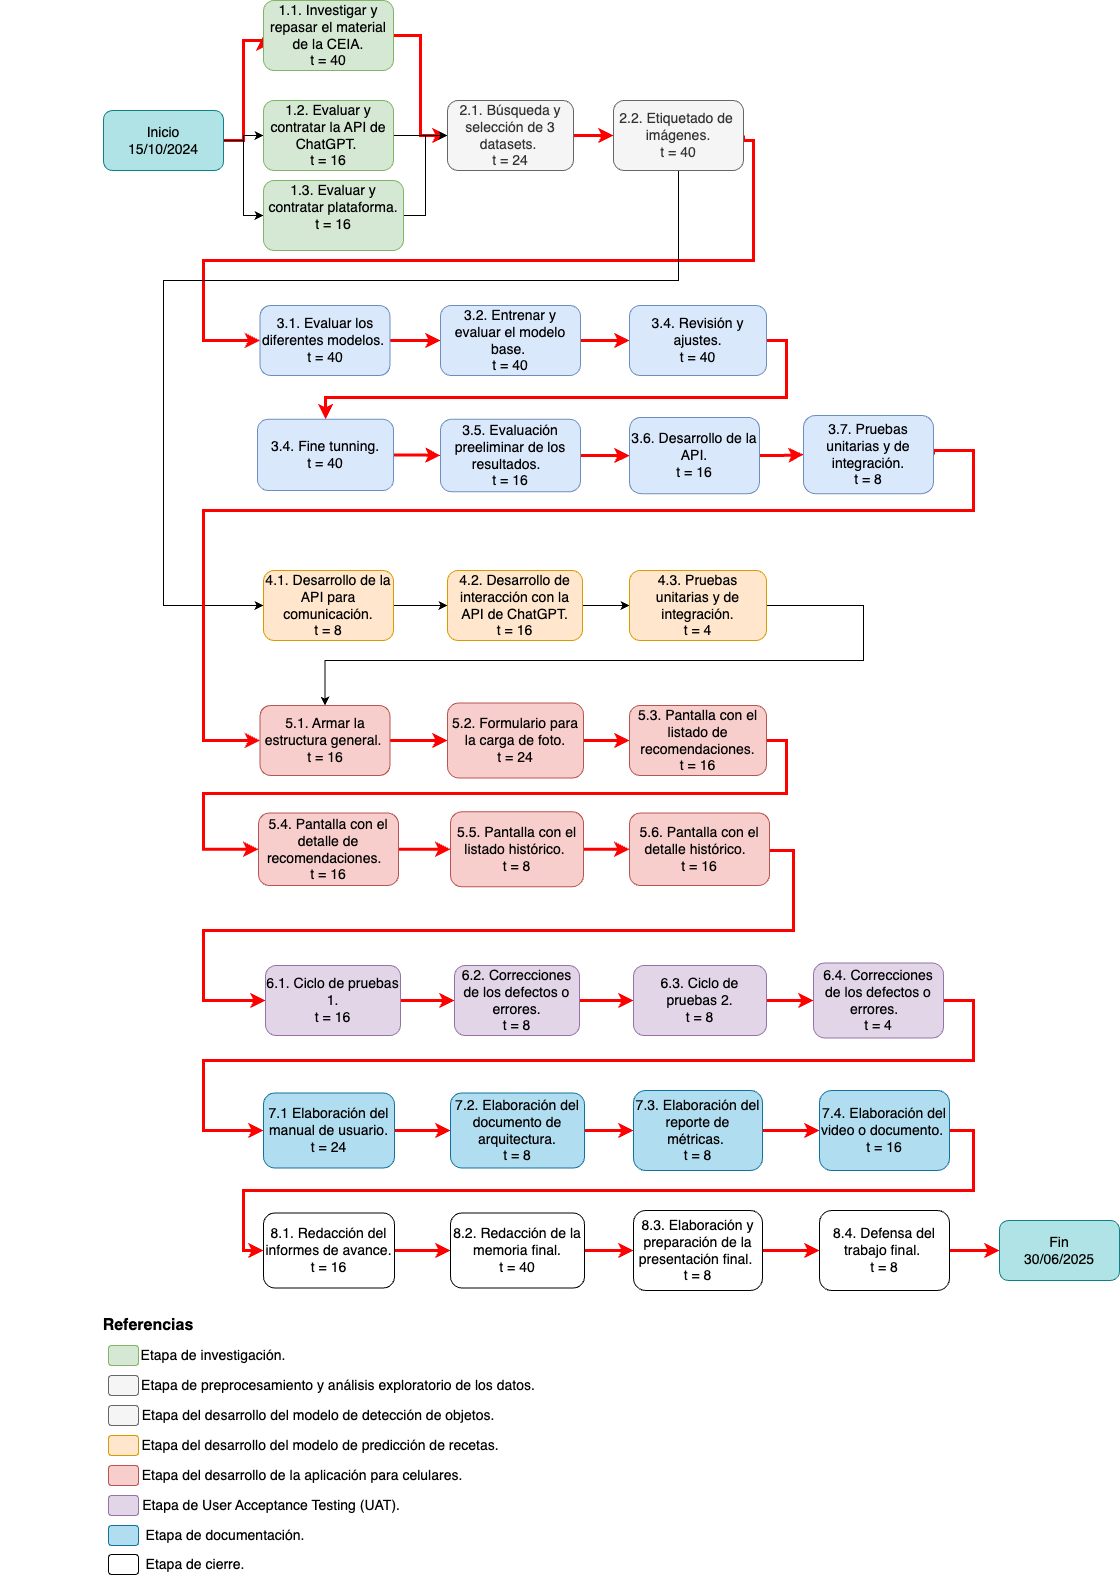
\includegraphics[width=1\textwidth]{./AoN.png}
\caption{Diagrama de \textit{Activity on Node}.}
\label{fig:AoN}
\end{figure}
\newpage
\section{11. Diagrama de Gantt}
\label{sec:gantt}

\begin{figure}[H]
\centering 
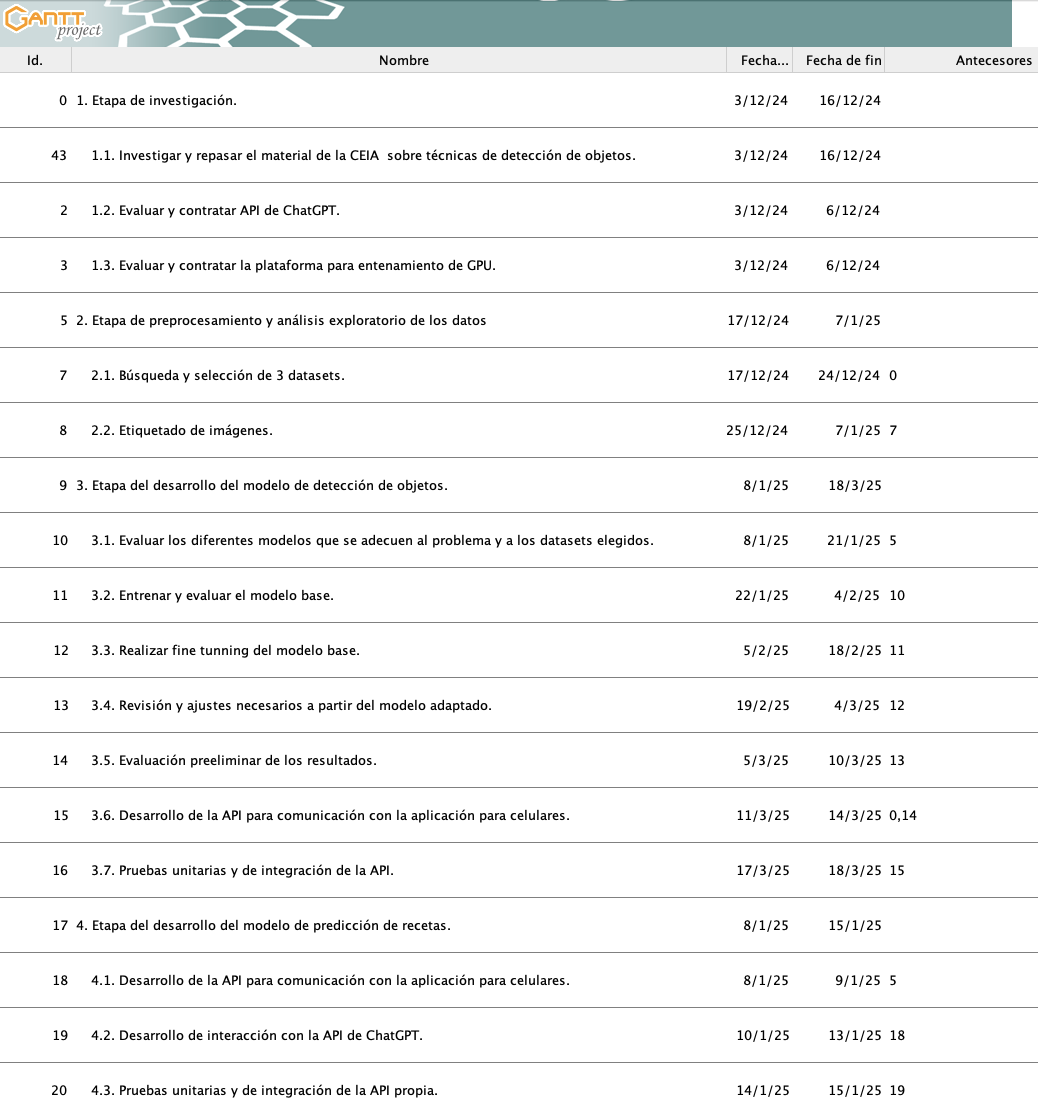
\includegraphics[width=1\textwidth]{./GanttActividades1.png}
\label{fig:AoN}
\end{figure}


\begin{figure}[H]
\centering 
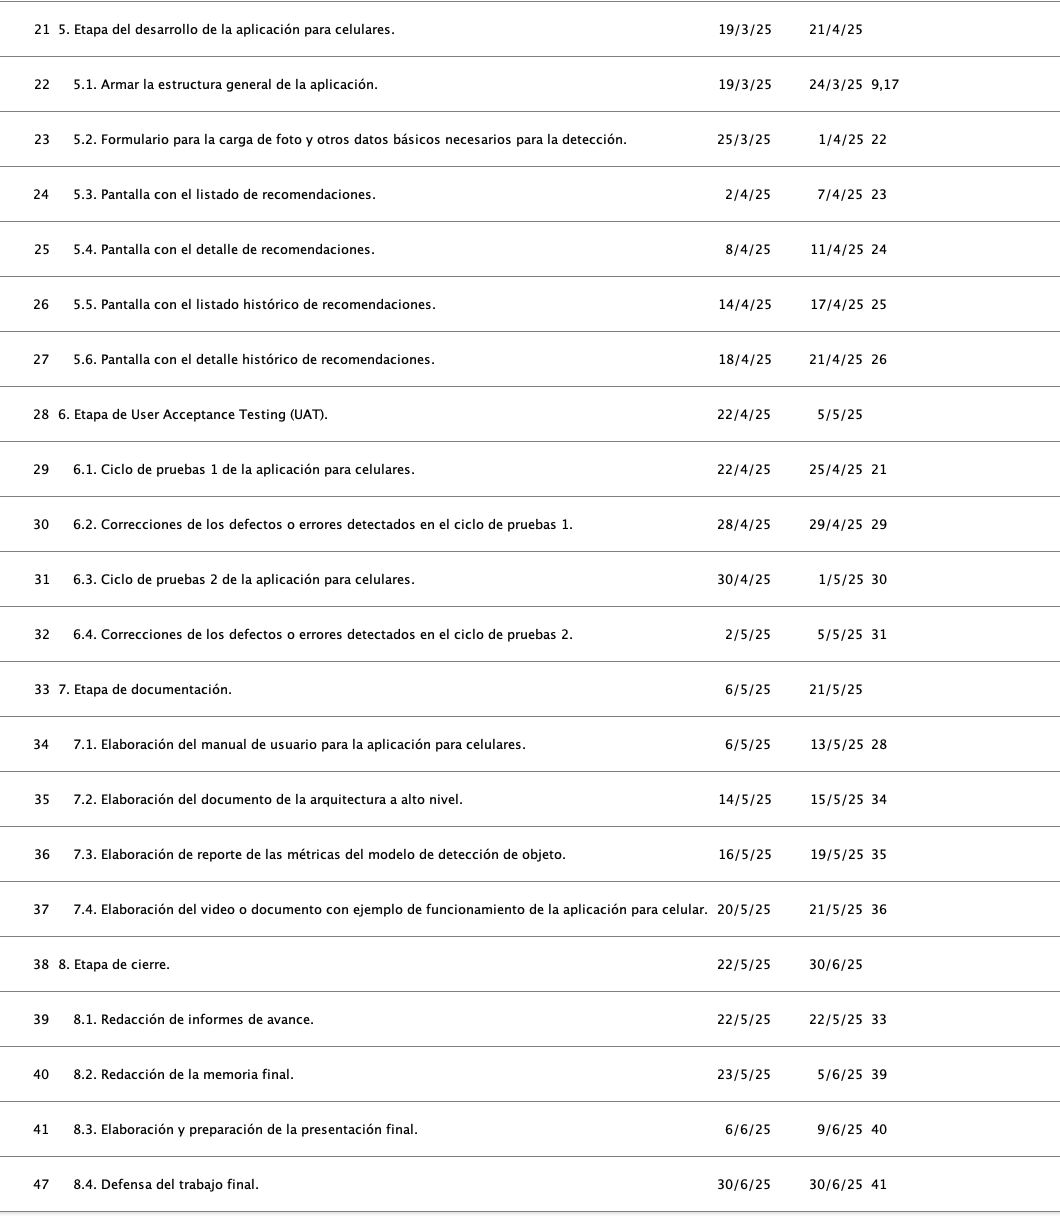
\includegraphics[width=1\textwidth]{./GanttActividades2.png}
\caption{EDT.}
\label{fig:AoN}
\end{figure}


\begin{landscape}
\begin{figure}[H]
\centering 
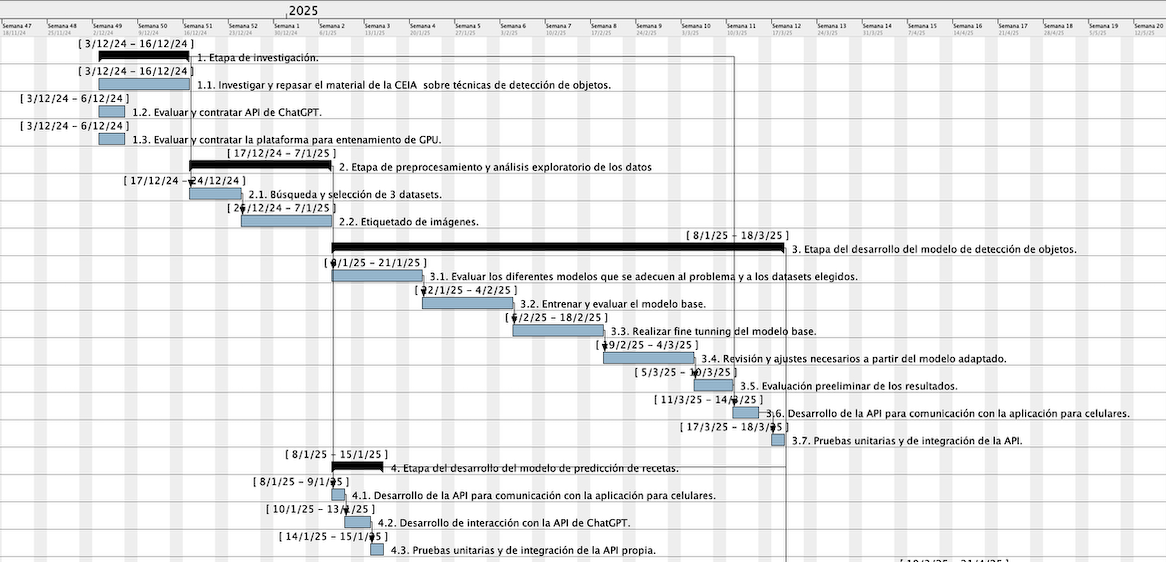
\includegraphics[width=1.55\textwidth]{./Gantt1.png}
\label{fig:AoN}
\end{figure}
\end{landscape}

\begin{landscape}
\begin{figure}[H]
\centering 
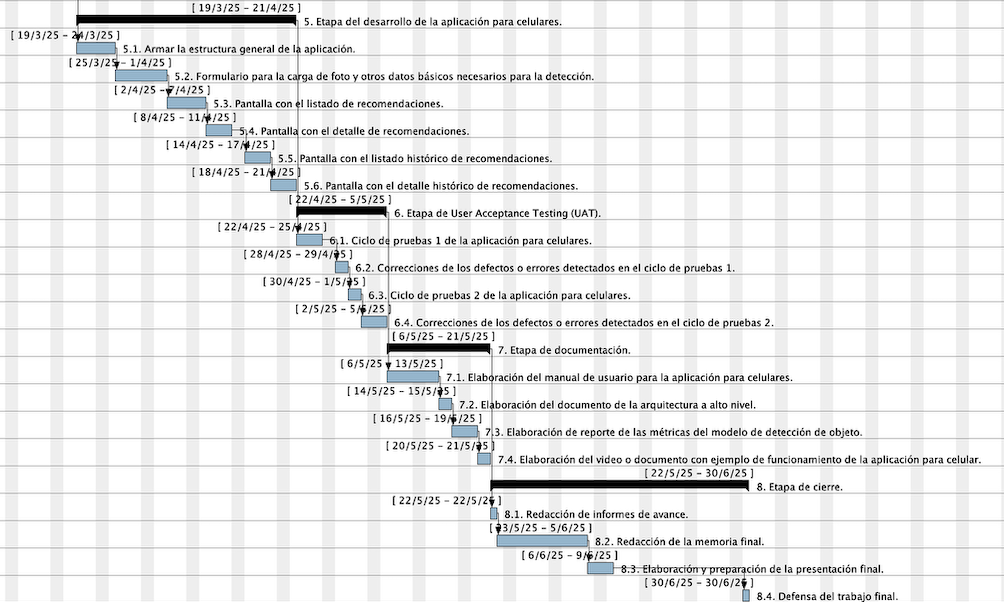
\includegraphics[width=1.5\textwidth]{./Gantt2.png}
\caption{Gantt}
\label{fig:AoN}
\end{figure}
\end{landscape}


\section{12. Presupuesto detallado del proyecto}
\label{sec:presupuesto}

\begin{table}[htpb]
\centering
\begin{tabularx}{\linewidth}{@{}|X|c|r|r|@{}}
\hline
\rowcolor[HTML]{C0C0C0} 
\multicolumn{4}{|c|}{\cellcolor[HTML]{C0C0C0}COSTOS DIRECTOS} \\ \hline
\rowcolor[HTML]{C0C0C0} 
Descripción &
  \multicolumn{1}{c|}{\cellcolor[HTML]{C0C0C0}Cantidad} &
  \multicolumn{1}{c|}{\cellcolor[HTML]{C0C0C0}Valor unitario} &
  \multicolumn{1}{c|}{\cellcolor[HTML]{C0C0C0}Valor total} \\ \hline
 
  Horas de ingeniería del responsable. &
  \multicolumn{1}{c|}{600} &
  \multicolumn{1}{c|}{ARS 90.000,00 } &
  \multicolumn{1}{c|}{ARS 54.000.000} \\ \hline
  Licencia mensual Google Colab Pro+ (USD 49,99). &
  \multicolumn{1}{c|}{6} &
  \multicolumn{1}{c|}{ARS 50.814,84} &
  \multicolumn{1}{c|}{ARS 304.889} \\ \hline
  
  Licencia mensual Chat GPT Pro (USD 19,99). &
  \multicolumn{1}{c|}{6} &
  \multicolumn{1}{c|}{ARS 20.319,84} &
  \multicolumn{1}{c|}{ARS 121.919} \\ \hline
  
  
\multicolumn{1}{|l|}{} &
   &
   &
   \\ \hline
\multicolumn{1}{|l|}{} &
   &
   &
   \\ \hline
\multicolumn{3}{|c|}{SUBTOTAL} &
  \multicolumn{1}{c|}{ARS 54.426.808} \\ \hline
\rowcolor[HTML]{C0C0C0} 
\multicolumn{4}{|c|}{\cellcolor[HTML]{C0C0C0}COSTOS INDIRECTOS} \\ \hline
\rowcolor[HTML]{C0C0C0} 
Descripción &
  \multicolumn{1}{c|}{\cellcolor[HTML]{C0C0C0}Cantidad} &
  \multicolumn{1}{c|}{\cellcolor[HTML]{C0C0C0}Valor unitario} &
  \multicolumn{1}{c|}{\cellcolor[HTML]{C0C0C0}Valor total} \\ \hline
\multicolumn{1}{|l|}{20	\% de los costos directos.} & 1
   & ARS 10.885.362
   & ARS 10.885.362
   \\ \hline
\multicolumn{1}{|l|}{} &
   &
   &
   \\ \hline
\multicolumn{1}{|l|}{} &
   &
   &
   \\ \hline
\multicolumn{3}{|c|}{SUBTOTAL} &
  \multicolumn{1}{c|}{ARS 10.885.362} \\ \hline
\rowcolor[HTML]{C0C0C0}
\multicolumn{3}{|c|}{TOTAL} & ARS 65.312.170
   \\ \hline
\end{tabularx}%
\end{table}

Nota: la tasa de cambio  utilizada fue la del Banco de la Nación Argentina (BNA), tipo vendedor, al 9 de noviembre de 2024 (USD 1 = ARS 1.016,50). 

\section{13. Gestión de riesgos}
\label{sec:riesgos}
Se han identificado los siguientes riesgos: 

Riesgo 1: no contar con suficientes imágenes de calidad para entrenar el modelo de detección de objetos.
\begin{itemize}
\item Severidad (S): tener una buena calidad de imágenes es crucial para un buen entrenamiento de modelos de inteligencia artificial. Sin datos de calidad, las métricas de cualquier modelo son extremadamente pobres. (10)
\item Probabilidad de ocurrencia (O): con frecuencia los datasets disponibles en los sitios web son limitados en cuanto a la cantidad y calidad de imágenes. Adicionalmente, suelen tener poco ruido o diversidad, lo que los alejan de las imágenes reales que un usuario de la aplicación utilizará en la inferencia. (9)
\end{itemize}

Riesgo 2: falta de conocimientos técnicos para la realización del modelo de detección de objetos.
\begin{itemize}
\item Severidad (S): contar con conocimientos técnicos en modelos de visión por computadoras es fundamental para lograr métricas eficientes y eficaces. (7)
\item Probabilidad de ocurrencia (O):  el responsable ya cuenta con una base en la temática dado que cursó dos materias en la CEIA, sin embargo pueden no ser suficientes. (7)
\end{itemize}

Riesgo 3: no contar con dinero suficiente para afrontar el presupuesto del proyecto.
\begin{itemize}
\item Severidad (S): sin los recursos adecuados no se puede realizar el entrenamiento del módulo de detección de objetos y no será posible realizar la inferencia utilizando las API de Chat GPT. Existen recursos gratuitos que podrían soportar los requerimientos parcialmente. (9)
\item Probabilidad de ocurrencia (O): el responsable ya evaluó los costos que deberá incurrir y tiene el dinero ahorrado disponible para afrontarlos. (2)
\end{itemize}

Riesgo 4: no cumplir con los tiempos de finalización del proyecto.
\begin{itemize}
\item Severidad (S): el responsable tiene pensado continuar con la especialización en internet de las cosas, con lo que un atraso en el trabajo final conllevaría a un atraso en el comienzo de la nueva especialización. Dado que no tiene dedicación exclusiva, no puede hacer las dos cosas a la vez. La severidad no es tan alta ya que FIUBA abre cohortes de todas las especializaciones varias veces al año. (2)
\item Probabilidad de ocurrencia (O): el responsable trabaja \textit{fulltime} y se encuentra con proyectos importantes en la compañía para la que trabaja, requiriéndole horas extras para cumplir. (10)
\end{itemize}

Riesgo 5: no conseguir suficientes amigos y familiares que oficien como usuarios finales.
\begin{itemize}
\item Severidad (S): sin un buen \textit{testing} es probable que la calidad del producto final no sea la esperada. El responsable tiene conocimientos gastronómicos con lo que algunas pruebas podría hacerlas el mismo. La gastronomía no es una ciencia que requiere elevado conocimiento específico. (5)
\item Probabilidad de ocurrencia (O): muchos familiares y amigos ya se han comprometido de palabra con el responsable para realizar estas tareas. (2)
\end{itemize}



\begin{table}[htpb]
\centering
\begin{tabularx}{\linewidth}{@{}|X|c|c|c|c|c|c|@{}}
\hline
\rowcolor[HTML]{C0C0C0} 
Riesgo & S & O & RPN & S* & O* & RPN* \\ \hline
Riesgo 1: no contar con suficientes imágenes de calidad para entrenar el modelo de detección de objetos.      & 10   & 9  &  90   & 10   &  1  &   10   \\ \hline
Riesgo 2: falta de conocimientos técnicos para la realización del modelo de detección de objetos.     & 7  & 7  &  49   & 7   &  2  &    14  \\ \hline
Riesgo 3: no contar con dinero suficiente para afrontar el presupuesto del proyecto.       & 9  & 2  &   18  &    &    &      \\ \hline
Riesgo 4: no cumplir con los tiempos de finalización del proyecto.       &  2 & 10  &   20  &    &    &      \\ \hline
Riesgo 5: no conseguir suficientes amigos y familiares que oficien como usuarios finales.       & 5  &  2 &    10 &    &    &      \\ \hline
\end{tabularx}%
\end{table}

Criterio adoptado: se tomarán medidas de mitigación en los riesgos cuyos números de RPN
sean mayores a 45.

Nota: los valores marcados con (*) en la tabla corresponden luego de haber aplicado la
mitigación del riesgo.


\textbf{Plan de mitigación de los riesgos que originalmente excedan el RPN máximo establecido}\\\\
Riesgo 1: solicitar a amigos y familiares que saquen fotos de sus propias heladeras y así obtener un dataset. Adicionalmente, solicitar al director que colabore en la búsqueda de un dataset en aquellas páginas proveedoras de diferentes conjuntos de datos.

Nueva asignación de S y O, con su respectiva justificación:
\begin{itemize}
\item Severidad (S): la severidad no cambia ya que malos datos seguirán generando malos modelos. (10)
\item Probabilidad de ocurrencia (O): la probablidad de ocurrencia cae drásticamente ya que son imágenes que se pueden conseguir fácilmente por cualquier persona (solamente usando su dispositivo celular). (1)
\end{itemize}

Riesgo 2: conseguir un codirector con conocimientos en visión por computadoras y solicitar ayuda a graduados y colegas de la CEIA.

Nueva asignación de S y O, con su respectiva justificación:
\begin{itemize}
\item Severidad (S):  si aun con la ayuda de un codirector o colegas no se logra reforzar los conocimientos técnicos, la \textit{performance} del modelo será baja y no logrará buenas detecciones de alimentos. (7)
\item Probabilidad de ocurrencia (O): con la ayuda de varios especialistas en este tipo de modelos es poco probable llegar a malos modelos de detección. (2)
\end{itemize}


\section{14. Gestión de la calidad}
\label{sec:calidad}


A continuación, se enumeran los diez requerimientos más importantes del proyecto y su correspondiente procedimiento de verificación y validación. 

\begin{itemize} 

% Inicio Req 
\item Req \#1.1.1: se deben utilizar, al menos, 3 datasets de fotos de heladeras con alimentos o alimentos sueltos (por ejemplo arriba de una mesada).

\begin{itemize}
	\item Verificación: se deberá chequear que los 3 dataset provengan de diferentes accesos y autores. Pueden estar en el mismo repositorio o página web.
	\item Validación: se revisará con el orientador del trabajo final si los datasets son adecuados para el entrenamiento.
\end{itemize}
% Fin Req 

% Inicio Req 
\item Req \#1.1.5: el sistema, mediante el entrenamiento de un modelo de visión por computadoras, debe detectar alimentos en la imagen recibida y devolverlas en forma de lista.

\begin{itemize}
	\item Verificación: se deberán programar rutinas de \textit{testing} para observar si el algoritmo es capaz de detectar los alimentos presentes.
	\item Validación: se revisará con el orientador del trabajo final si la \textit{performance} del modelo es adecuada.
\end{itemize}
% Fin Req 

% Inicio Req 
\item Req \#1.2.1: el sistema debe recibir una lista de alimentos (ingredientes) y devolver una lista de posibles recetas de cocina que contengan algunos de estos. 

\begin{itemize}
	\item Verificación: se deberá programar rutinas de \textit{testing} para observar si la aplicación es capaz de devolver las recetas en el formato solicitado.
	\item Validación: se consultará con familiares y amigos que les guste cocinar para determinar si las recetas entregadas guardan relación con los alimentos enviados como parámetros.
\end{itemize}
% Fin Req 

% Inicio Req 
\item Req \#1.2.2: se debe desarrollar una interacción con las API de Chat GPT para que este realice la recomendación.

\begin{itemize}
	\item Verificación: se deberá programar rutinas de \textit{testing} para observar si la interacción con Chat GPT es correcta.
	\item Validación: se consultará con el orientador del trabajo final si el resultado de la interacción con la API es la esperada.
\end{itemize}
% Fin Req 

% Inicio Req 
\item Req \#1.3.2: el sistema debe listar las recomendaciones que el módulo de recomendación devuelva.

\begin{itemize}
	\item Verificación: se deberá realizar una captura de pantalla de la aplicación para celulares donde se muestre una lista de recomendaciones.
	\item Validación: se consultará con familiares y amigos que les guste cocinar si la lista brindada guarda relación con receta de alimentos.
\end{itemize}
% Fin Req 
% Inicio Req 
\item Req \#2.1: se debe poder contar con un repositorio en GitHub con todo el código fuente de todos los módulos.

\begin{itemize}
	\item Verificación: se deberá contar con un repositorio y se deberá realizar una captura de pantalla donde se muestre una carpeta con todos los módulos del proyecto.
	\item Validación: el orientador del trabajo final revisará el código fuente del repositorio y determinará si es correcto o no.
\end{itemize}
% Fin Req 

% Inicio Req 
\item Req \#2.4: los diferentes módulos deben estar organizados en docker containers.

\begin{itemize}
	\item Verificación: se deberán agregar los archivos \textit{dockerfiles} y \textit{dockercompose} e imprimir una captura de pantalla de dichos archivos.
	\item Validación: el orientador del trabajo final revisará el código fuente y determinará si tiene los archivos necesarios para la gestión de los módulos utilizando docker containers.
\end{itemize}
% Fin Req 

% Inicio Req 
\item Req \#3.1: se debe elaborar un diagrama a alto nivel con el diseño de la arquitectura del sistema.

\begin{itemize}
	\item Verificación: se debe realizar un documento que tiene que estar disponible en el repositorio de código.
	\item Validación: el orientador del trabajo final revisará el documento de diseño alojado en el repositorio y determinará si tiene el formato y contenido correcto.
\end{itemize}
% Fin Req 

% Inicio Req 
\item Req \#3.2: el usuario debe poder contar con un manual de usuario de la aplicación para dispositivos celulares.

\begin{itemize}
	\item Verificación: se debe realizar un manual que tiene que estar disponible en el repositorio.
	\item Validación: el orientador del trabajo final revisará el manual alojado en el repositorio y determinará si tiene el formato y contenido esperado para un manual de usuario.
\end{itemize}
% Fin Req 

% Inicio Req 
\item Req \#4.1: el usuario final debe evaluar y certificar la aplicación a desarrollar.

\begin{itemize}
	\item Verificación: se debe contar con la aprobación formal por medio de un correo electrónico del usuario final.
	\item Validación: el director del trabajo final debe revisar el correo electrónico y determinar si la aplicación a desarrollar fue aprobada por el usuario.
\end{itemize}
% Fin Req 



\end{itemize}




\section{15. Procesos de cierre}    
\label{sec:cierre}


\begin{itemize}
	\item Pautas de trabajo que se seguirán para analizar si se respetó el Plan de Proyecto original:
	 \begin{itemize}
	 \item Responsable: Ing. Fabricio Denardi.
	 \item Procedimiento:
	 \begin{enumerate}
	 	\item Revisar el proyecto original y sus objetivos.
	 	\item Comprobar los entregables realizados con los planificados en el plan original.
	 	\item Evaluar los recursos utilizados respecto a los planificados.
	 	\item Identificar cambios y desvíos en el alcance, tiempo y presupuesto.
	 	\item Documentar los cambios y desvíos en caso que los haya habido. 	
	 \end{enumerate}
	 \end{itemize}
	\item Identificación de las técnicas y procedimientos útiles e inútiles que se emplearon, los problemas que surgieron y cómo se solucionaron:
	\begin{itemize}
	 \item Responsable: Ing. Fabricio Denardi.
	 \item Procedimiento:
	 \begin{enumerate}
	 	\item Revisar las técnicas y procedimientos que se utilizaron en el proyecto.
	 	\item Identificar aquellas que han sido efectivas y contribuyeron al éxito del proyecto.
	 	\item Identificar las que, por el contrario, resultaron ineficaces y causaron problemas.
	 	\item Realizar una videollamada con el director del trabajo final en donde se discutan estas técnicas y procedimiento. Adicionalmente, en esta videollamada se deben establecer las lecciones aprendidas que dejó este proyecto.
	 	\item Elaborar un informe de las lecciones aprendidas discutidas en la videollamada.
	 \end{enumerate}
	 
	 \end{itemize}
	\item Indicar quién organizará el acto de agradecimiento a todos los interesados, y en especial, al equipo de trabajo y colaboradores:
	 \begin{itemize}
	 \item Responsable: Ing. Fabricio Denardi.
	 \item Procedimiento:
	 \begin{enumerate}
	 	\item Organizar un acto de agradecimiento en donde participen todos los interesados. Este acto se debe hacer mediante una videoconferencia.
	 \end{enumerate}
	 
	 \end{itemize}
	 
	 \item Realizar una presentación y demostración pública del proyecto ante los jurados. 
	  \begin{itemize}
	 \item Responsable: Ing. Fabricio Denardi.
	 \item Procedimiento:
	 \begin{enumerate}
	 \item El responsable debe coordinar con la FUIBA la presentación y demostración pública.
	 	\item El responsable debe presentar su proyecto ante los jurados y el público en general.
	 \end{enumerate}
	 \end{itemize}
\end{itemize}



\end{document}